% ____________________________________________________________________________
% Differentials and interpretation

\section{Tables for the differential cross section measurements}
\label{sec:tables}

Tables~\ref{tab:numbers_pth_smH}--\ref{tab:numbers_ptjet} show the measured differential cross sections for the considered observables.

\begin{table}[h!]
    \caption{
        Differential cross sections (pb/GeV) for the observable $\pth$.
        }
    \label{tab:numbers_pth_smH}
    \scriptsize
    \begin{center}
    \begin{tabular}{|l|c|c|c|c|c|c|c|c|c|}
    \hline
    $\pth$ (GeV)                         & 0-15                      & 15-30                   & 30-45                     & 45-80                      & 80-120                      & 120-200                      & 200-350                                                & 350-600                                                              & $>$600                                                               \\ 
 \hline 
$\hboson \rightarrow \photon\photon$ & $1.0 \, {}^{+0.3}_{-0.3}$ & $1 \, {}^{+0.3}_{-0.3}$ & $0.5 \, {}^{+0.2}_{-0.2}$ & $0.3 \, {}^{+0.1}_{-0.1}$  & $0.1 \, {}^{+0.05}_{-0.05}$ & $0.03 \, {}^{+0.01}_{-0.01}$ & $0.01 \, {}^{+2.8 \cdot 10^{-3}}_{-2.5 \cdot 10^{-3}}$ & $-3.4 \cdot 10^{-5} \, {}^{+3.8 \cdot 10^{-4}}_{-3.1 \cdot 10^{-4}}$ & $-1.9 \cdot 10^{-4} \, {}^{+2.4 \cdot 10^{-4}}_{-2.4 \cdot 10^{-4}}$ \\ 
 \hline 
$\hboson \rightarrow \zboson\zboson$ & $0.7 \, {}^{+0.3}_{-0.3}$ & $1 \, {}^{+0.4}_{-0.3}$ & \multicolumn{2}{c|}{$0.4 \, {}^{+0.1}_{-0.1}$}         & \multicolumn{2}{c|}{$0.08 \, {}^{+0.03}_{-0.02}$}          & \multicolumn{3}{c|}{$3.3 \cdot 10^{-4} \, {}^{+2.6 \cdot 10^{-3}}_{-2.6 \cdot 10^{-3}}$}                                                                                                             \\ 
 \hline 
$\hboson \rightarrow \bquark\bquark$ & -                         & -                       & -                         & -                          & -                           & -                            & -                                                      & $9.6 \cdot 10^{-4} \, {}^{+1.2 \cdot 10^{-3}}_{-1.2 \cdot 10^{-3}}$  & $1.1 \cdot 10^{-4} \, {}^{+1.2 \cdot 10^{-4}}_{-1.1 \cdot 10^{-4}}$  \\ 
 \hline 
Combination                          & $0.8 \, {}^{+0.2}_{-0.2}$ & $1 \, {}^{+0.2}_{-0.3}$ & $0.6 \, {}^{+0.2}_{-0.2}$ & $0.3 \, {}^{+0.1}_{-0.09}$ & $0.1 \, {}^{+0.05}_{-0.04}$ & $0.03 \, {}^{+0.01}_{-0.01}$ & $0.01 \, {}^{+2.6 \cdot 10^{-3}}_{-2.4 \cdot 10^{-3}}$ & $-2.8 \cdot 10^{-6} \, {}^{+3.7 \cdot 10^{-4}}_{-2.8 \cdot 10^{-4}}$ & $5.8 \cdot 10^{-5} \, {}^{+1.0 \cdot 10^{-4}}_{-1.0 \cdot 10^{-4}}$  \\
    \hline
    \end{tabular}
    \end{center}
    \end{table}

\begin{table}[h!]
    \caption{
        Differential cross sections (pb/GeV) for the observable $\pth$, with non-\ggh production modes fixed to their SM prediction.
        }
    \label{tab:numbers_pth_ggH}
    \scriptsize
    \begin{center}
    \begin{tabular}{|l|c|c|c|c|c|c|c|c|c|}
    \hline
    $\pth$ (GeV) & 0-15                      & 15-30                   & 30-45                     & 45-80                      & 80-120                      & 120-200                      & 200-350                                                             & 350-600                                                              & $>$600                                                              \\ 
 \hline 
Combination  & $0.8 \, {}^{+0.2}_{-0.2}$ & $1 \, {}^{+0.2}_{-0.3}$ & $0.5 \, {}^{+0.2}_{-0.2}$ & $0.2 \, {}^{+0.1}_{-0.09}$ & $0.1 \, {}^{+0.05}_{-0.04}$ & $0.02 \, {}^{+0.01}_{-0.01}$ & $8.3 \times 10^{-3} \, {}^{+2.6 \times 10^{-3}}_{-2.4 \times 10^{-3}}$ & $-1.6 \times 10^{-4} \, {}^{+3.4 \times 10^{-4}}_{-2.6 \times 10^{-4}}$ & $3.5 \times 10^{-5} \, {}^{+5.8 \times 10^{-5}}_{-5.7 \times 10^{-5}}$ \\
    \hline
    \end{tabular}
    \end{center}
    \end{table}


\begin{table}[h!]
    \caption{
        Differential cross sections (pb) for the observable $\njets$.
        }
    \label{tab:numbers_njets}
    \scriptsize
    \begin{center}
    \begin{tabular}{|l|c|c|c|c|c|}
    \hline
    $\njets$                             & 0                                                                & 1                                                                & 2                                                                 & 3                                                                & $\ge$ 4                                                            \\ 
 \hline 
$\hboson \rightarrow \photon\photon$ & $5.0 \cdot 10^{1} \, {}^{+8.5 \cdot 10^{0}}_{-8.1 \cdot 10^{0}}$ & $1.4 \cdot 10^{1} \, {}^{+5.1 \cdot 10^{0}}_{-4.9 \cdot 10^{0}}$ & $4.8 \cdot 10^{-1} \, {}^{+2.7 \cdot 10^{0}}_{-2.7 \cdot 10^{0}}$ & $3.1 \cdot 10^{0} \, {}^{+2.0 \cdot 10^{0}}_{-2.0 \cdot 10^{0}}$ & $1.3 \cdot 10^{0} \, {}^{+8.8 \cdot 10^{-1}}_{-9.3 \cdot 10^{-1}}$ \\ 
 \hline 
$\hboson \rightarrow \zboson\zboson$ & $4.1 \cdot 10^{1} \, {}^{+9.1 \cdot 10^{0}}_{-8.0 \cdot 10^{0}}$ & $8.7 \cdot 10^{0} \, {}^{+5.2 \cdot 10^{0}}_{-4.3 \cdot 10^{0}}$ & $6.9 \cdot 10^{0} \, {}^{+3.7 \cdot 10^{0}}_{-3.0 \cdot 10^{0}}$  & \multicolumn{2}{c|}{$1.2 \cdot 10^{0} \, {}^{+2.1 \cdot 10^{0}}_{-2.1 \cdot 10^{0}}$}                                                 \\ 
 \hline 
Combination                          & $4.7 \cdot 10^{1} \, {}^{+6.2 \cdot 10^{0}}_{-6.4 \cdot 10^{0}}$ & $1.1 \cdot 10^{1} \, {}^{+3.7 \cdot 10^{0}}_{-3.4 \cdot 10^{0}}$ & $3.5 \cdot 10^{0} \, {}^{+1.9 \cdot 10^{0}}_{-1.7 \cdot 10^{0}}$  & $1.8 \cdot 10^{0} \, {}^{+1.7 \cdot 10^{0}}_{-1.5 \cdot 10^{0}}$ & $1.2 \cdot 10^{0} \, {}^{+8.3 \cdot 10^{-1}}_{-8.8 \cdot 10^{-1}}$ \\
    \hline
    \end{tabular}
    \end{center}
    \end{table}

\begin{table}[h!]
    \caption{
        Differential cross sections (pb) for the observable $\absy$.
        }
    \label{tab:numbers_absy}
    \scriptsize
    \begin{center}
    \begin{tabular}{|l|c|c|c|c|c|c|}
    \hline
    $\absy$                              & 0-0.15                                                           & 0.15-0.3                                                         & 0.3-0.6                                                          & 0.6-0.9                                                          & 0.9-1.2                                                          & 1.2-2.5                                                          \\ 
 \hline 
$\hboson \rightarrow \photon\photon$ & $4.2 \cdot 10^{1} \, {}^{+1.1 \cdot 10^{1}}_{-1.1 \cdot 10^{1}}$ & $3.9 \cdot 10^{1} \, {}^{+1.2 \cdot 10^{1}}_{-1.1 \cdot 10^{1}}$ & $3.1 \cdot 10^{1} \, {}^{+9.0 \cdot 10^{0}}_{-7.5 \cdot 10^{0}}$ & $2.8 \cdot 10^{1} \, {}^{+9.1 \cdot 10^{0}}_{-8.7 \cdot 10^{0}}$ & $2.4 \cdot 10^{1} \, {}^{+1.2 \cdot 10^{1}}_{-1.0 \cdot 10^{1}}$ & $1.8 \cdot 10^{1} \, {}^{+7.4 \cdot 10^{0}}_{-7.2 \cdot 10^{0}}$ \\ 
 \hline 
$\hboson \rightarrow \zboson\zboson$ & $3.9 \cdot 10^{1} \, {}^{+1.7 \cdot 10^{1}}_{-1.4 \cdot 10^{1}}$ & $3.5 \cdot 10^{1} \, {}^{+1.8 \cdot 10^{1}}_{-1.4 \cdot 10^{1}}$ & $3.4 \cdot 10^{1} \, {}^{+1.1 \cdot 10^{1}}_{-9.8 \cdot 10^{0}}$ & $4.5 \cdot 10^{1} \, {}^{+1.3 \cdot 10^{1}}_{-1.1 \cdot 10^{1}}$ & $1.3 \cdot 10^{1} \, {}^{+8.9 \cdot 10^{0}}_{-6.8 \cdot 10^{0}}$ & $1.3 \cdot 10^{1} \, {}^{+6.7 \cdot 10^{0}}_{-5.4 \cdot 10^{0}}$ \\ 
 \hline 
Combination                          & $4.1 \cdot 10^{1} \, {}^{+9.1 \cdot 10^{0}}_{-8.9 \cdot 10^{0}}$ & $3.8 \cdot 10^{1} \, {}^{+9.7 \cdot 10^{0}}_{-9.2 \cdot 10^{0}}$ & $3.2 \cdot 10^{1} \, {}^{+7.0 \cdot 10^{0}}_{-6.0 \cdot 10^{0}}$ & $3.5 \cdot 10^{1} \, {}^{+7.1 \cdot 10^{0}}_{-6.6 \cdot 10^{0}}$ & $1.7 \cdot 10^{1} \, {}^{+7.4 \cdot 10^{0}}_{-6.5 \cdot 10^{0}}$ & $1.5 \cdot 10^{1} \, {}^{+5.1 \cdot 10^{0}}_{-4.7 \cdot 10^{0}}$ \\
    \hline
    \end{tabular}
    \end{center}
    \end{table}

\begin{table}[h!]
    \caption{
        Differential cross sections (pb/GeV) for the observable $\ptjet$.
        }
    \label{tab:numbers_ptjet}
    \scriptsize
    \begin{center}
    \begin{tabular}{|l|c|c|c|c|c|}
    \hline
    $\ptjet$ (GeV)                       & 30-55                                                               & 55-95                                                               & 95-120                                                              & 120-200                                                              & $>$200                                                              \\ 
 \hline 
$\hboson \rightarrow \photon\photon$ & $1.6 \cdot 10^{-1} \, {}^{+2.0 \cdot 10^{-1}}_{-2.1 \cdot 10^{-1}}$ & $2.0 \cdot 10^{-1} \, {}^{+9.2 \cdot 10^{-2}}_{-9.3 \cdot 10^{-2}}$ & $1.3 \cdot 10^{-1} \, {}^{+9.5 \cdot 10^{-2}}_{-9.2 \cdot 10^{-2}}$ & $1.5 \cdot 10^{-5} \, {}^{+1.8 \cdot 10^{-2}}_{-1.7 \cdot 10^{-2}}$  & $2.9 \cdot 10^{-2} \, {}^{+9.1 \cdot 10^{-3}}_{-9.2 \cdot 10^{-3}}$ \\ 
 \hline 
$\hboson \rightarrow \zboson\zboson$ & $4.8 \cdot 10^{-1} \, {}^{+2.4 \cdot 10^{-1}}_{-2.0 \cdot 10^{-1}}$ & $7.7 \cdot 10^{-2} \, {}^{+8.8 \cdot 10^{-2}}_{-6.9 \cdot 10^{-2}}$ & \multicolumn{3}{c|}{$8.0 \cdot 10^{-2} \, {}^{+5.9 \cdot 10^{-2}}_{-4.4 \cdot 10^{-2}}$}                                                                                                                         \\ 
 \hline 
Combination                          & $3.2 \cdot 10^{-1} \, {}^{+1.4 \cdot 10^{-1}}_{-1.3 \cdot 10^{-1}}$ & $1.3 \cdot 10^{-1} \, {}^{+7.7 \cdot 10^{-2}}_{-6.1 \cdot 10^{-2}}$ & $1.1 \cdot 10^{-1} \, {}^{+8.4 \cdot 10^{-2}}_{-8.1 \cdot 10^{-2}}$ & $-4.2 \cdot 10^{-3} \, {}^{+1.7 \cdot 10^{-2}}_{-1.6 \cdot 10^{-2}}$ & $2.7 \cdot 10^{-2} \, {}^{+8.7 \cdot 10^{-3}}_{-8.9 \cdot 10^{-3}}$ \\
    \hline
    \end{tabular}
    \end{center}
    \end{table}


% ____________________________________________________________________________
\clearpage
\section{Correlation matrices for the combinations of differential observables}
\label{sec:binToBinCorrelationMatrices}

Figs.~\ref{fig:corrMat_pth}--\ref{fig:corrMat_ptjet} show the correlation matrices for the considered observables.

\begin{figure}[hbtp]
  \begin{center}
    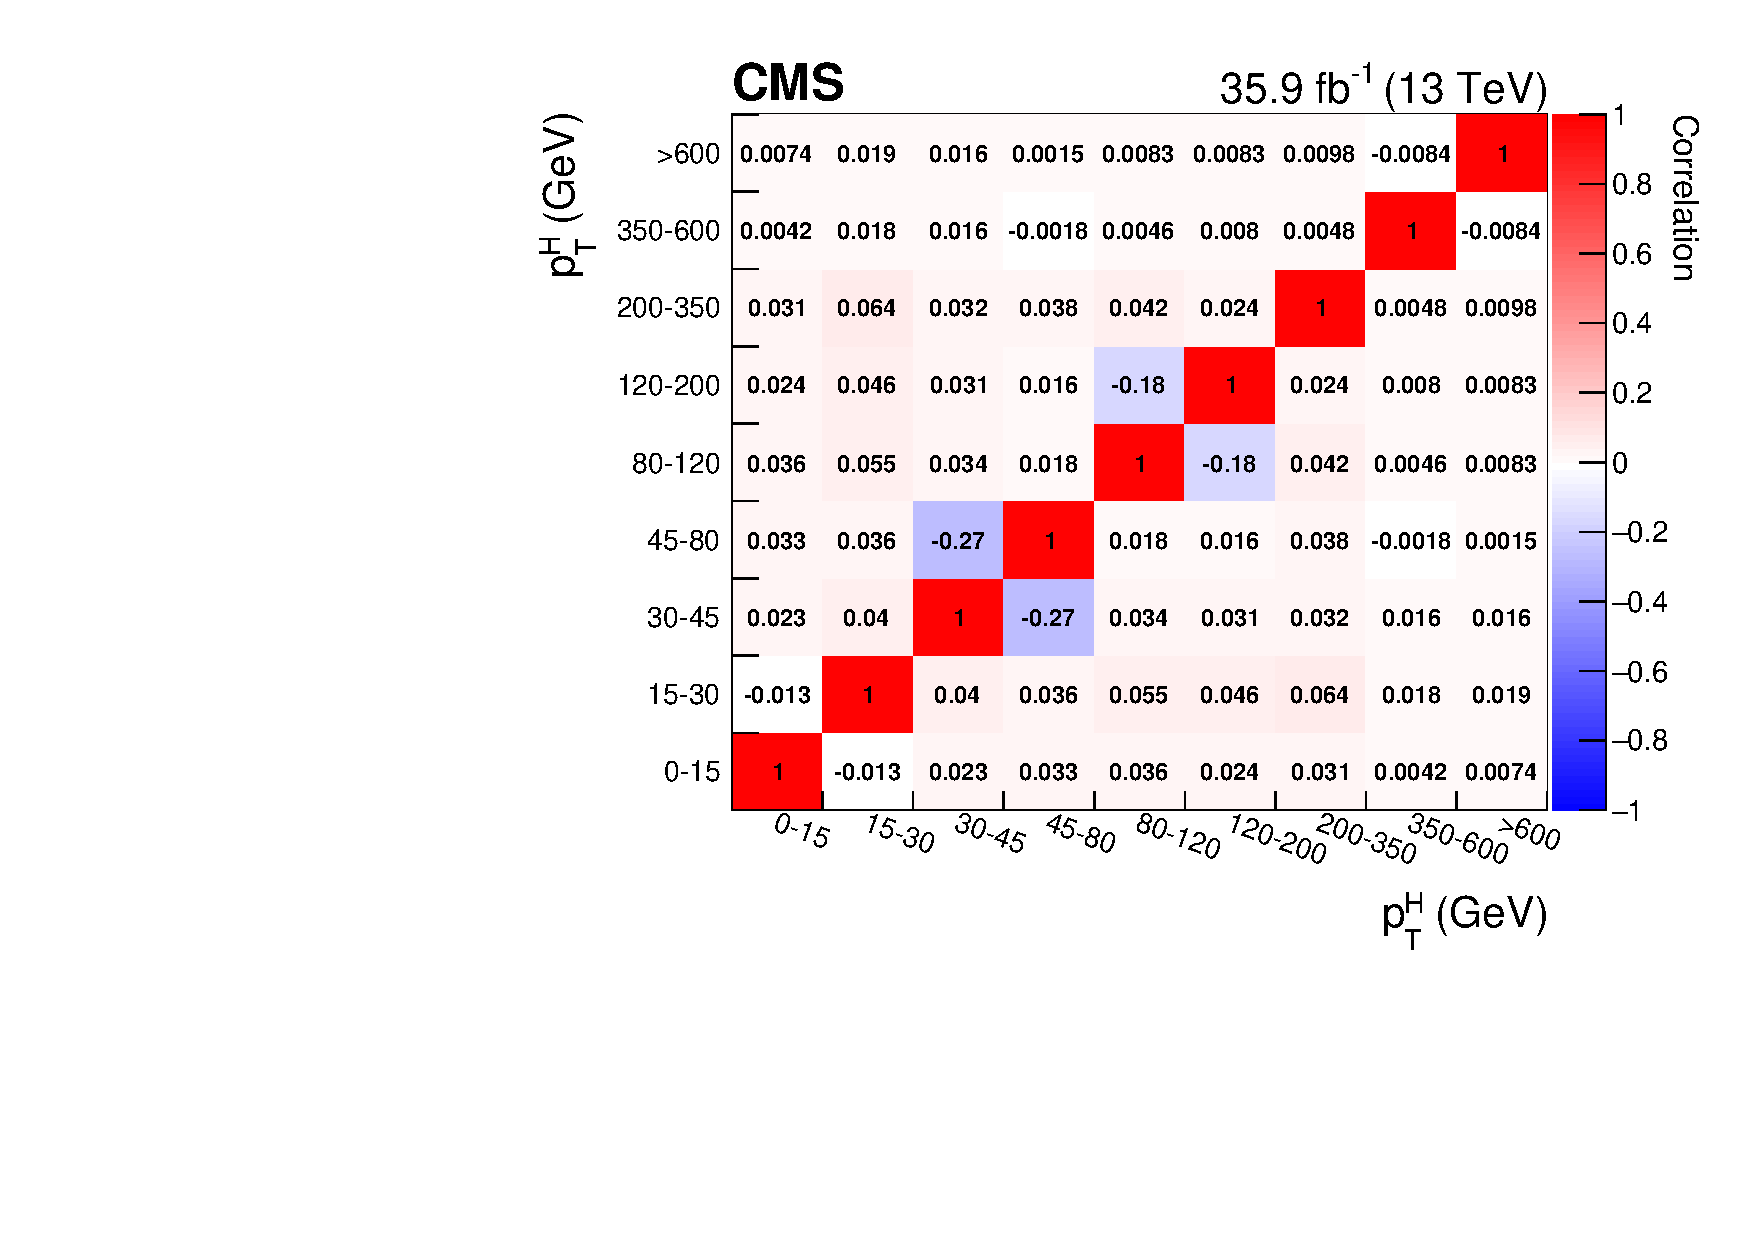
\includegraphics[width=0.49\linewidth]{img/differentials/appendix/corrmat_pth_smH.pdf}
    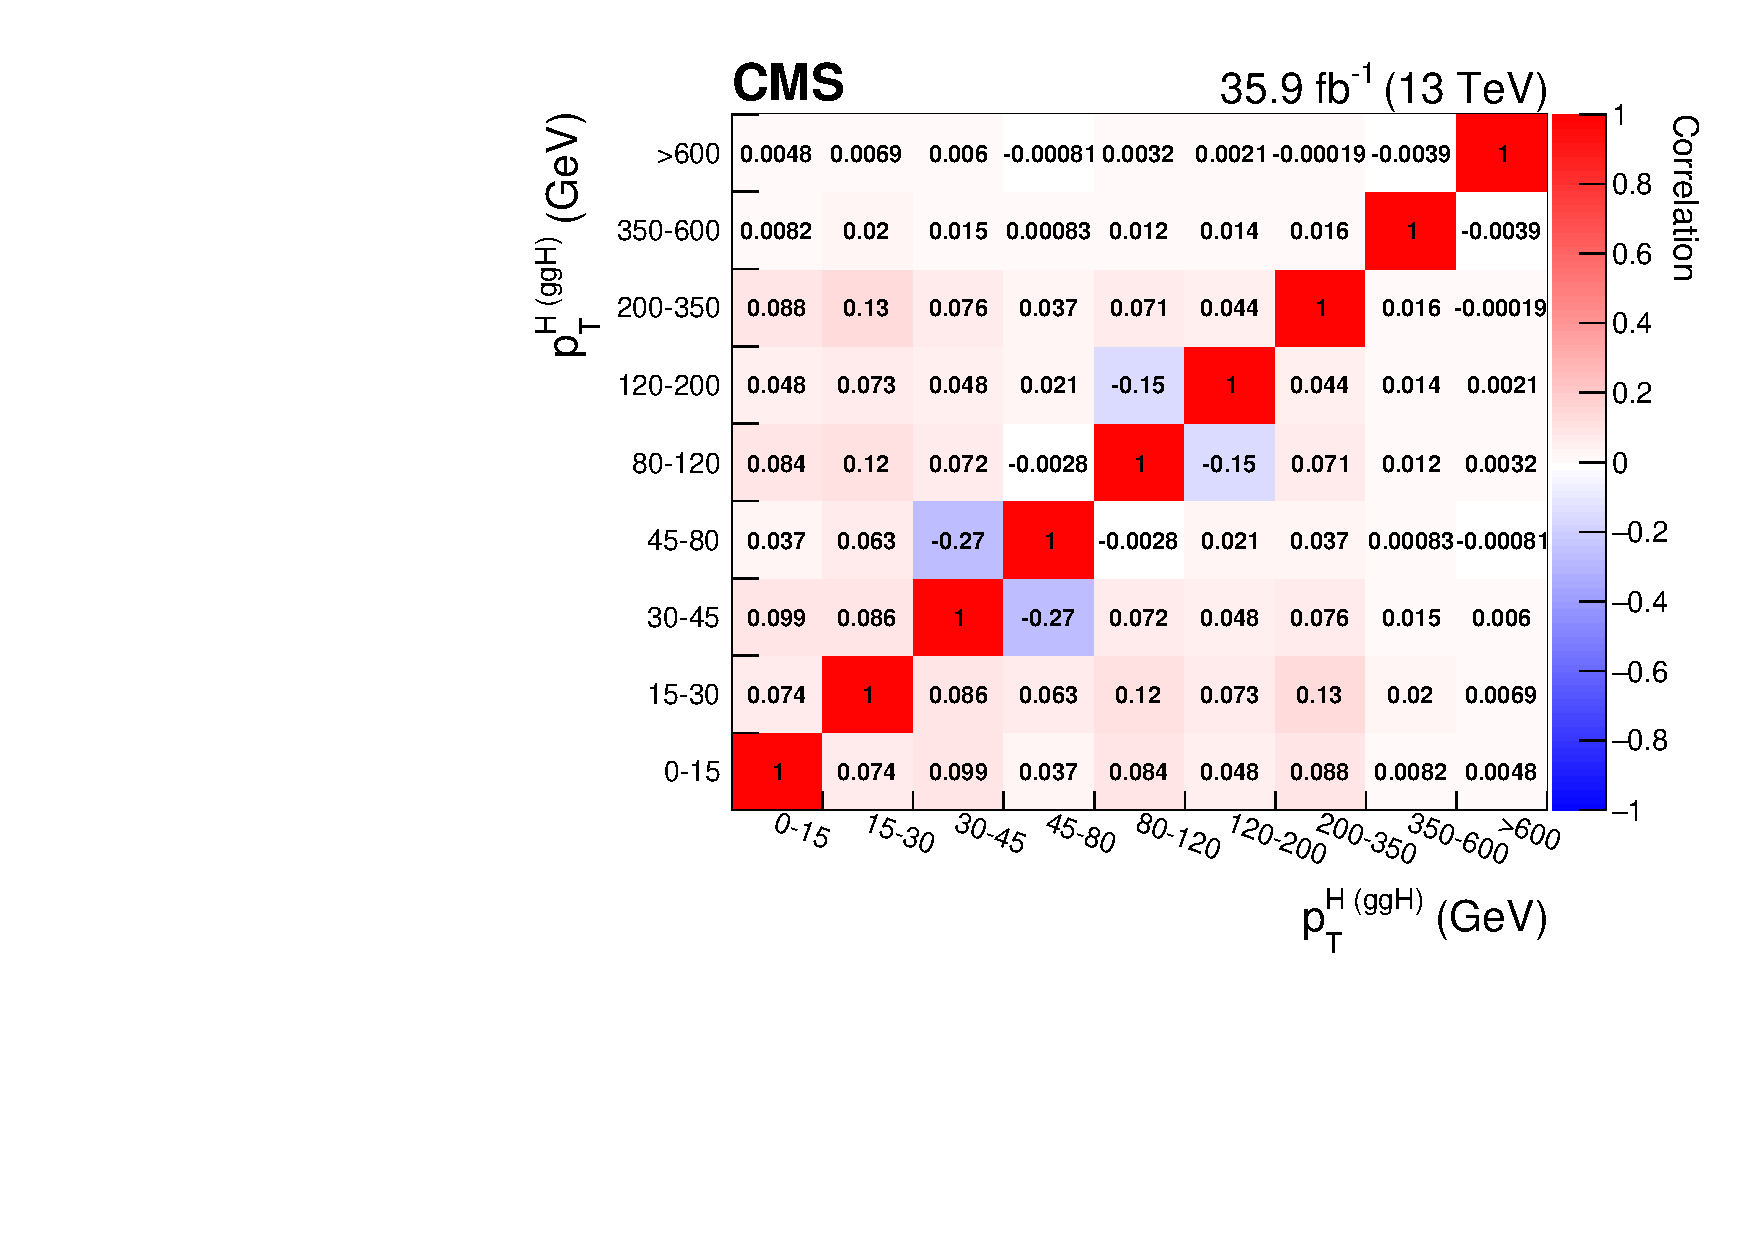
\includegraphics[width=0.49\linewidth]{img/differentials/appendix/corrmat_pth_ggH.pdf}
    \caption{
         Bin-to-bin correlation matrix of the $\pth$ spectrum (left) and of the $\pth$ spectrum while keeping the non-\ggh contributions fixed to the SM expectation (right).
        }
    \label{fig:corrMat_pth}
  \end{center}
\end{figure}

\begin{figure}[hbtp]
  \begin{center}
    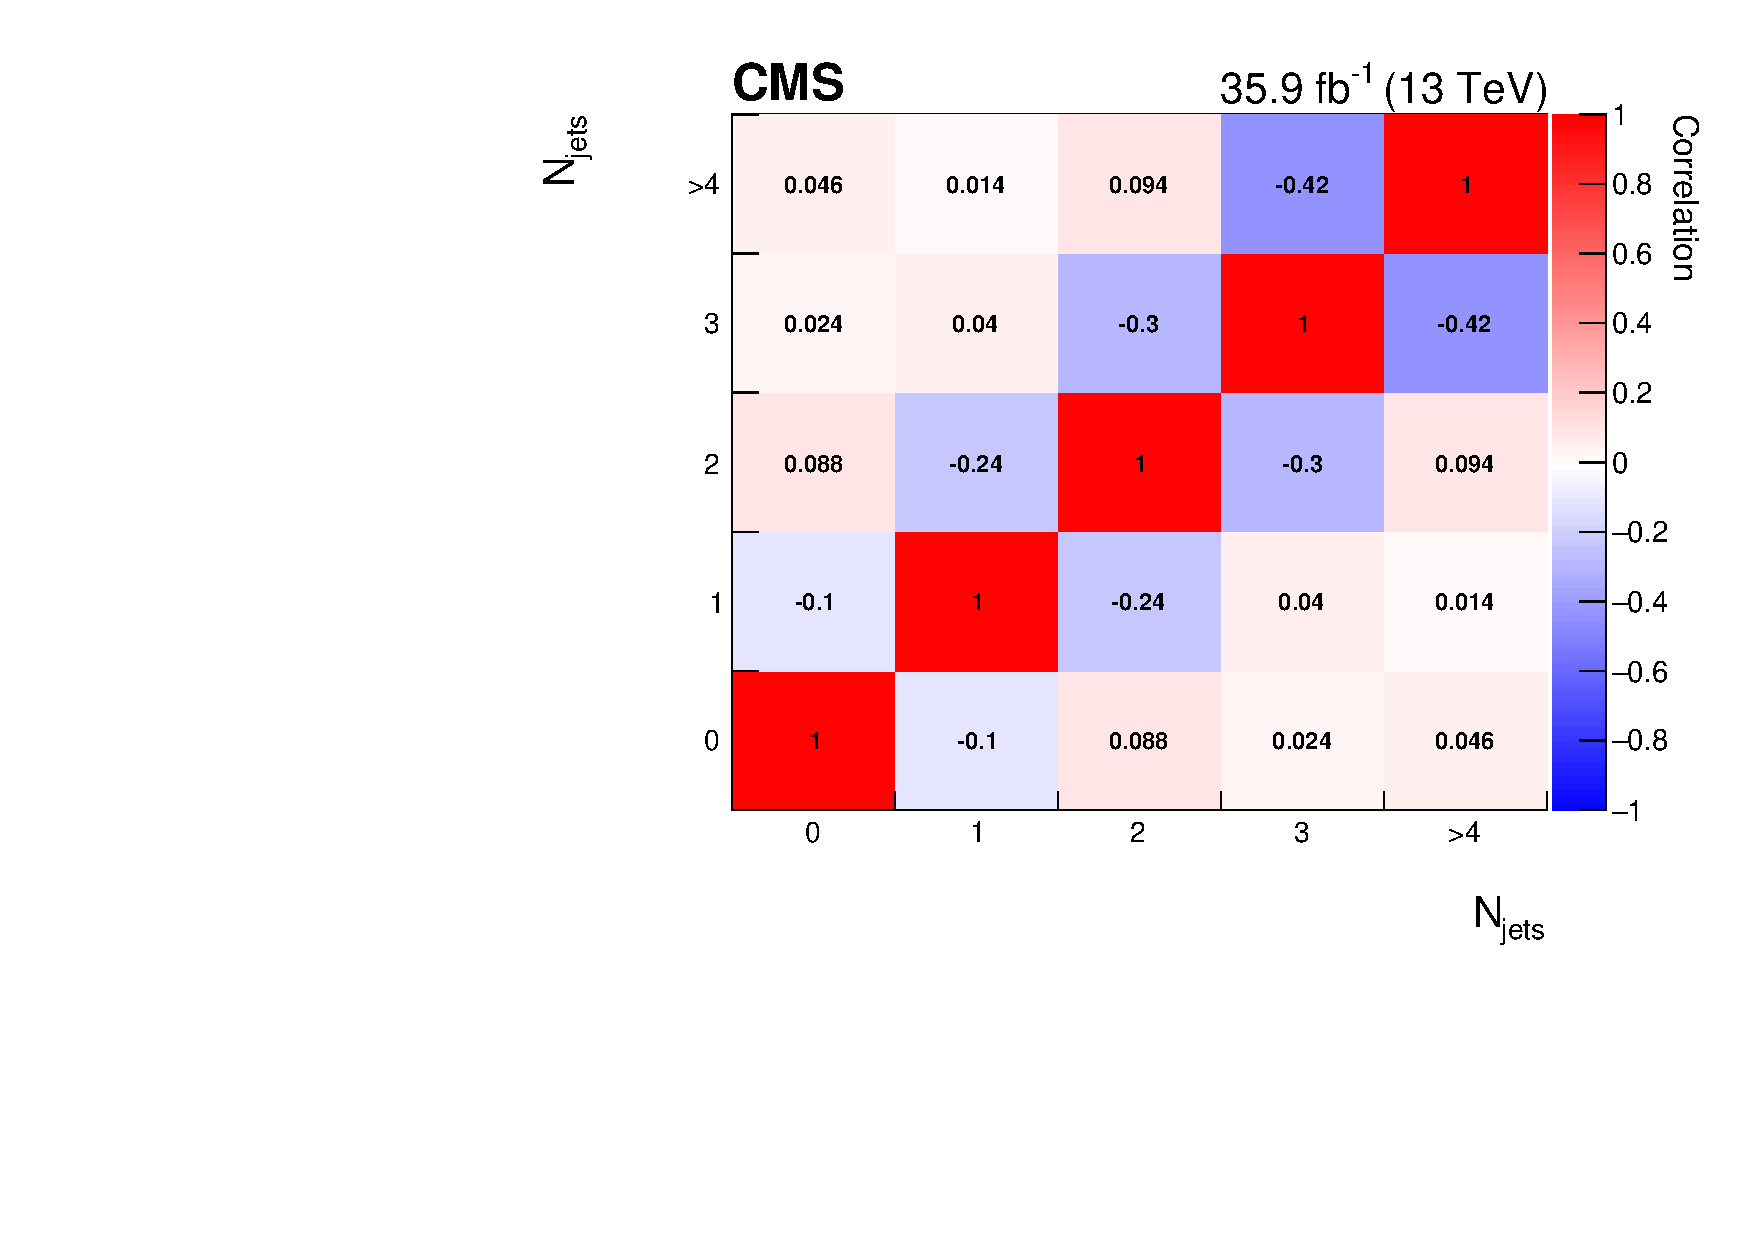
\includegraphics[width=0.49\linewidth]{img/differentials/appendix/corrmat_njets.pdf}
    \caption{
        Bin-to-bin correlation matrix of the $\njets$ spectrum.
        }
    \label{fig:corrMat_njets}
  \end{center}
\end{figure}

\begin{figure}[hbtp]
  \begin{center}
    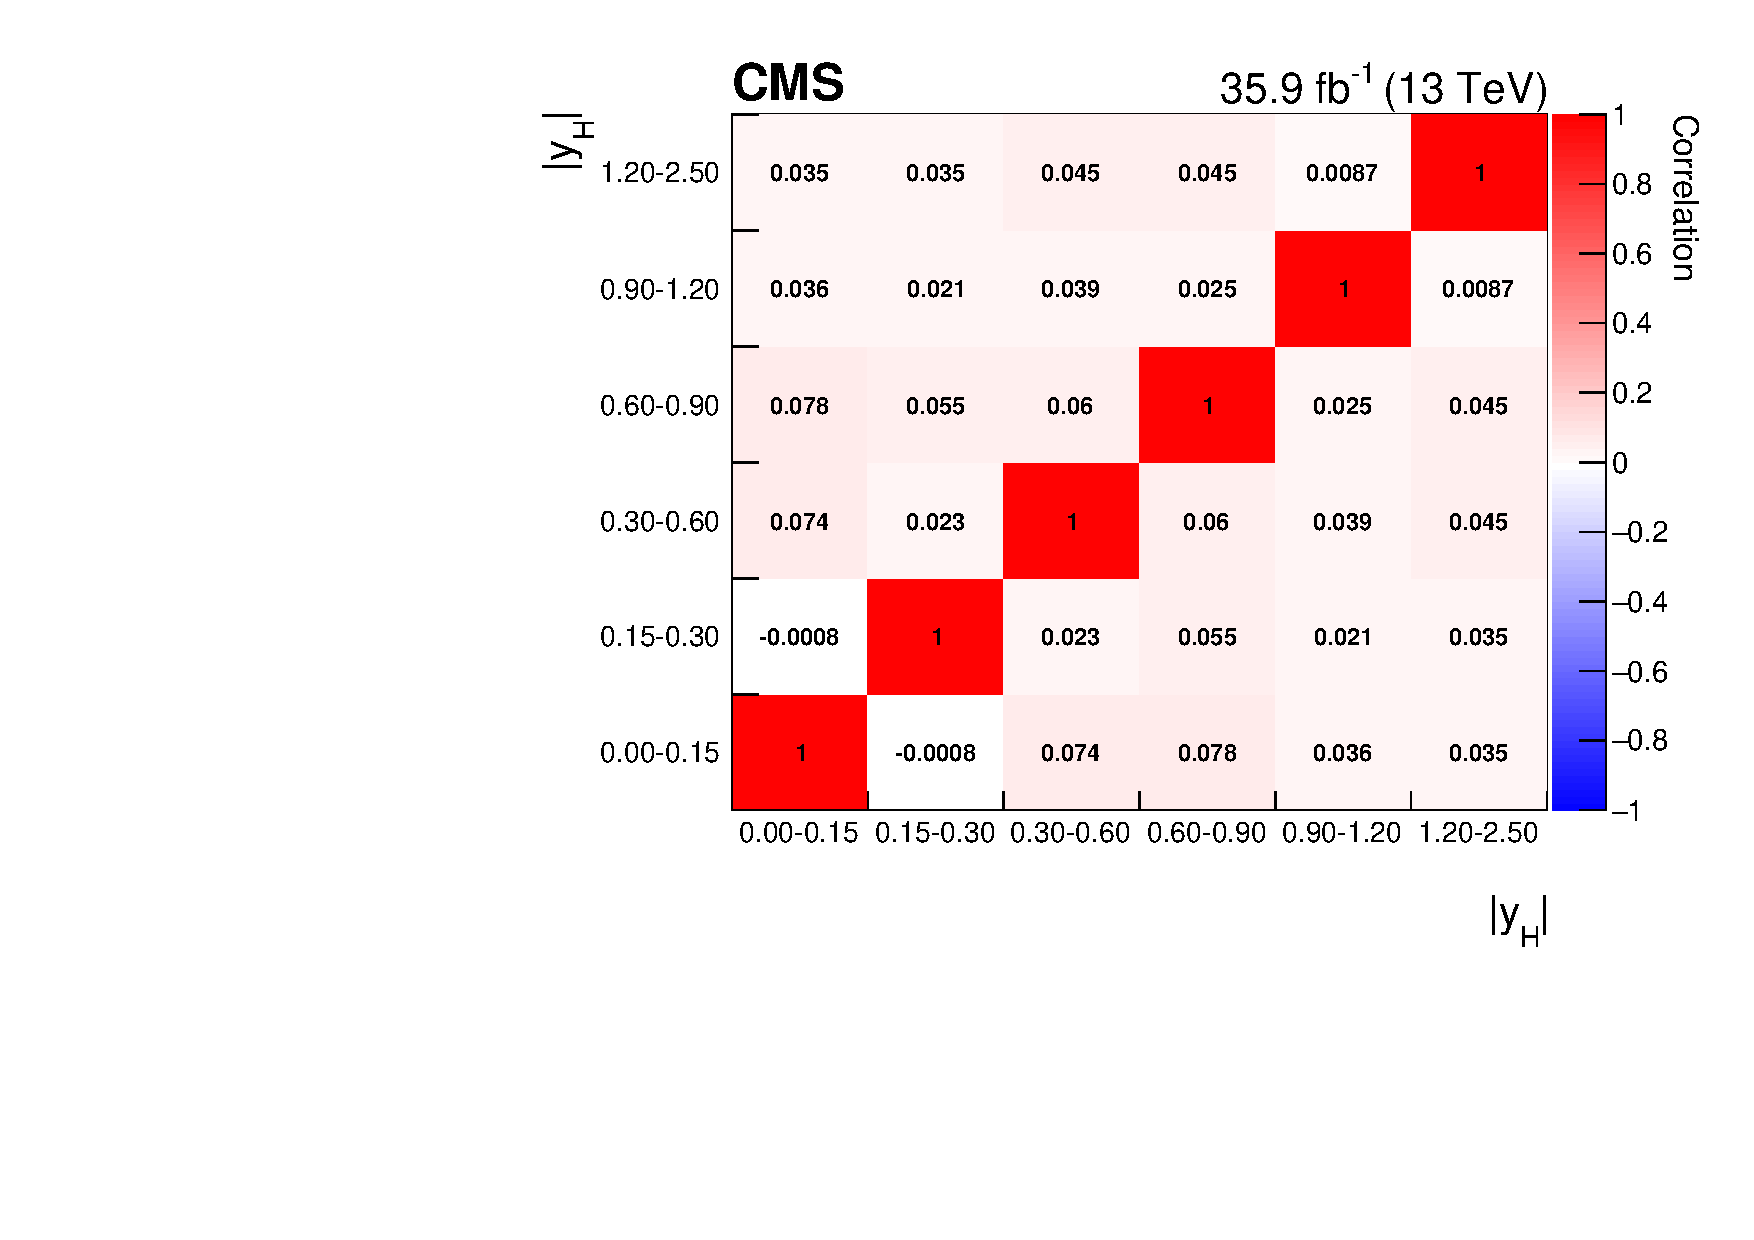
\includegraphics[width=0.49\linewidth]{img/differentials/appendix/corrmat_rapidity.pdf}
    \caption{
        Bin-to-bin correlation matrix of the $\absy$ spectrum.
        }
    \label{fig:corrMat_absy}
  \end{center}
\end{figure}

\begin{figure}[hbtp]
  \begin{center}
    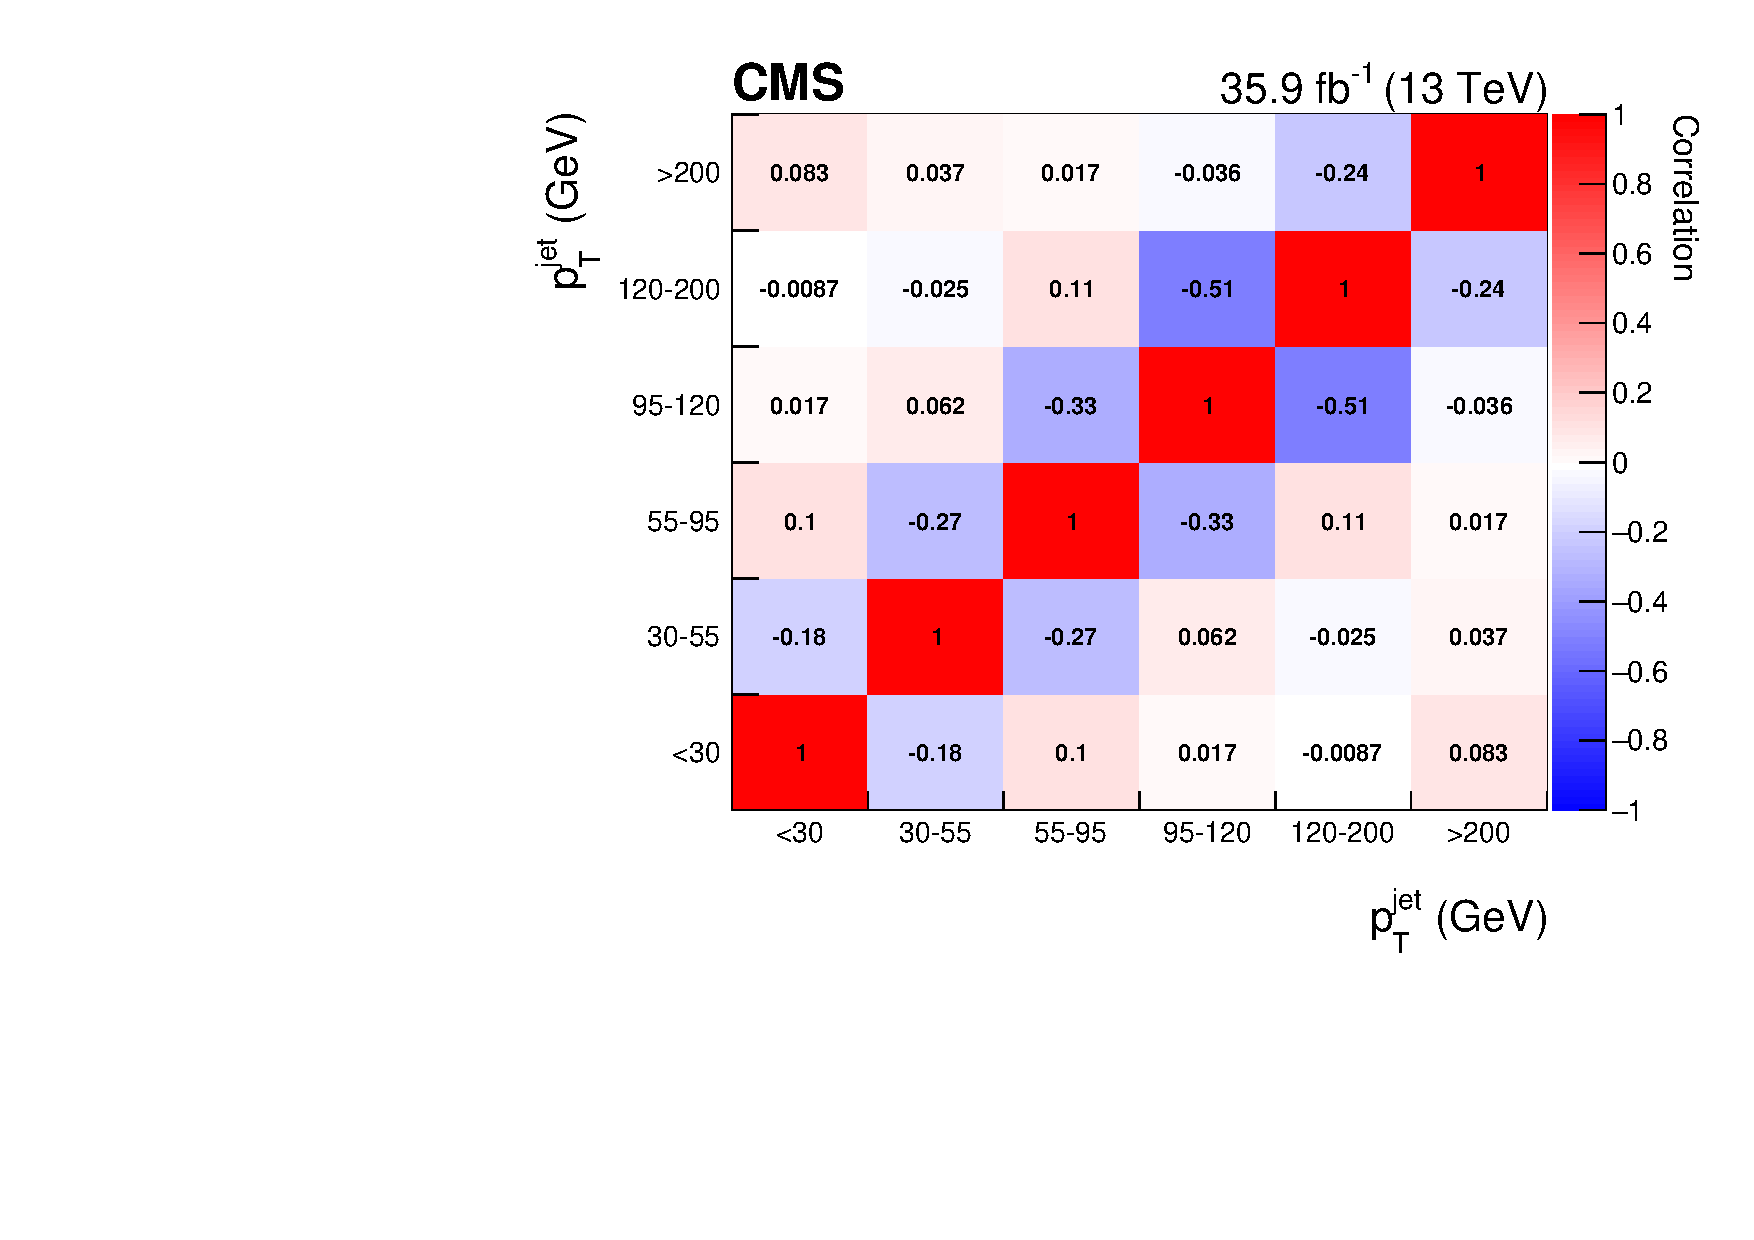
\includegraphics[width=0.49\linewidth]{img/differentials/appendix/corrmat_ptjet.pdf}
    \caption{
        Bin-to-bin correlation matrix of the $\ptjet$ spectrum.
        }
    \label{fig:corrMat_ptjet}
  \end{center}
\end{figure}

% ____________________________________________________________________________
% alphas
\subimport{alphas/}{appendix}